\documentclass[a4paper,11pt]{report}
\usepackage[T1]{fontenc}
\usepackage[utf8]{inputenc}
\usepackage{lmodern}
\usepackage{color}
\usepackage{graphicx}
\graphicspath{ {images/} }
\usepackage{hyperref}

\title{Enron Fraud Detection Project}
\author{Neil Seas}

\begin{document}

\maketitle
\tableofcontents

\begin{abstract}
This document answers the
    \href{https://docs.google.com/document/d/1NDgi1PrNJP7WTbfSUuRUnz8yzs5nGVTSzpO7oeNTEWA/pub?embedded=true}{questions}
    posed in the Project \textbf{Identify Fraud from Enron Email} in the Udacity Data Analyst Nanodegree program.
\end{abstract}

\chapter{Questions}
\section{Question 1}

The goal of this project is to use the financial and email features in the Enron
data set to identify persons-of-interest in the Enron fraud investigation.
Machine learning is an ideal tool for a classification problem such as
this.  There are several \textbf{classification} algorithms that we can apply to
this problem such as \textbf{e.g. Naive Bayes or Decision Trees} to name only two.
In addition to classification algorithms, machine learning provides other tools
such as feature selection \textbf{e.g. SelectKBest}, which can help to find the features
with the most predictive power.  We can also utilize dimensionality reduction
techniques such as principle component analysis, which combines the existing
features into a smaller set of features.

There were two outliers that I removed from the data set.  The first was the
\textbf{TOTAL} row of the financial features.  The second outlier was the
\textbf{THE TRAVEL AGENCY IN THE PARK}.  These records were removed using the
\textbf{pop} method on the data\_dict dictionary.  Given the small data set, these
outliers were identified by manually scanning the information provided in
\textbf{enron61702insiderpay.pdf}

After removing outliers, there are 144 total records in the data set and 18
persons-of-interest.  There are 19 features provided in the data set and a
number of features are mostly empty (e.g.
loan advances, director fees, and restricted stock deferred), but given that we
are using SelectKBest for our feature selection we do not preemptively remove
these from the data.  The table below shows the top five features with the
highest percentage of values that are NaN.

\begin{center}
    \begin{tabular}{|| l c ||}
        \hline Feature & Pct NaN \\
        \hline\hline
        loan advances & 97.9167 \\
        \hline
        director fees & 88.8889 \\
        \hline
        restricted stock deferred & 88.1944 \\
        \hline
        deferral payments & 73.6111 \\
        \hline
        deferred income & 66.6667 \\
        \hline
    \end{tabular}
\end{center}

\section{Question 2}

\textbf{Feature Selection} \\

The features utilized in the final model are \textbf{bonus},
\textbf{exercised\_stock\_options}, \textbf{salary}, \textbf{total\_stock\_value}
and two engineered features \textbf{bonus\_salary\_gap} and
\textbf{pct\_email\_poi}. Initially, I attempted to remove features by looking
at pairwise correlations.  I was assuming that would allow me to see the
strength of the relationship with the poi labels as well as provide an overview
of which features were highly correlated and therefore unlikely to add
additional value to the model.  While this approach was successful in
getting the precision and recall above the required .30 it did not perform as
well as using \textbf{SelectKBest}.

I ran SelectKBest across the range of possible values of k (i.e. 1-21) in the
context of GridSearchCV.  The resulting value of k was six.  It is clear from the
table and charts below that these six features have the highest scores and are also
associated with the highest level of precision and recall.

The feature scores are as follows: \\

\begin{center}
    \begin{tabular}{|| l c ||}
        \hline Feature & Score \\
        \hline\hline
        bonus & 20.79225 \\
        \hline
        exercised\_stock\_options & 24.81508 \\
        \hline
        salary & 18.28968 \\
        \hline
        total\_stock\_value & 24.18290 \\
        \hline
        bonus\_salary\_gap & 18.11560 \\
        \hline
        pct\_email\_to\_poi & 16.40971 \\
        \hline
    \end{tabular}
\end{center}

\begin{figure}[!h]
    \centering
    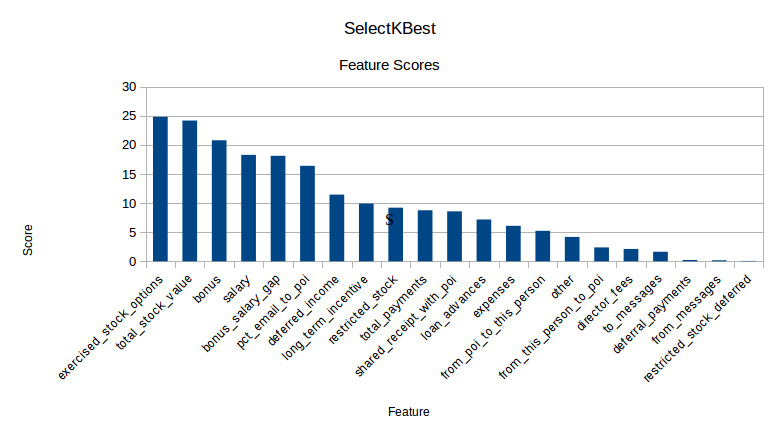
\includegraphics[scale=.6]{feature_scores.png}
    \caption{SelectKBest Feature Scores}
\end{figure}

\begin{figure}[!h]
    \centering
    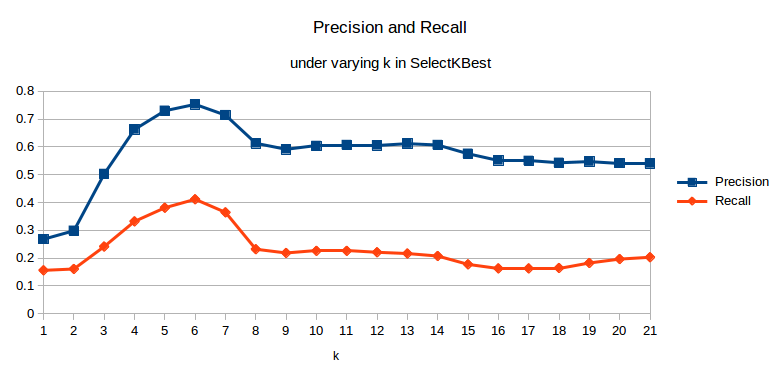
\includegraphics[scale=.6]{precision_recall.png}
    \caption{Precision and Recall}
\end{figure}

\textbf{Engineered Features} \\

Two engineered features were used in the final model.  The first, the percentage
of a persons email sent to a person of interest, was discussed in the course
materials.  This feature is simply the number of emails sent to a POI out of the
total number of sent emails (i.e. from\_this\_person\_to\_poi / from\_messages).  The
second feature is the \textbf{bonus\_salary\_gap}.  This feature measures the
difference between a persons bonus and their salary in dollars.  The intuition behind this
feature was that there may be POIs whose bonus was disproportionate to their
salary and this could provide additional information.  Perhaps there were lower
ranking employees whose silence was paid for with a large bonus.  Initially, I
constructed this feature as the bonus to salary ratio, but I switched to the
nominal difference between bonus and salary as it improved the K-nearest
neighbor result. \\

\textbf{Scaling} \\

I did use scaling (StandardScalar) when testing each algorithm, but particularly
in the case of the final KNN model it lowered the precision and recall
significantly.

\section{Question 3}
  
My final model utilizes the K-nearest neighbors algorithm as it gave the highest
levels for both precision and recall across all of the algorithms that I tested.
I started with Naive Bayes and Decision Trees to get an idea of where the
precision and recall were without making any transformations on the data or
adding additional features.  I then tested SVM and KNN algorithms in the same
manner.  Below is a summary of the base algorithms that were tested.

\textbf{Summary of Base Models} \\
\begin{center}
    \begin{tabular}{|| l c c c||}
        \hline Algorithm & Precision & Recall & F1 \\
        \hline\hline
        Naive Bayes & .22604 & .39500 & .28753 \\
        \hline
        Decision Tree & .25155 & .22300 & .23642 \\
        \hline
        SVM & N/A & N/A & N/A \\
        \hline
        KNN & .60870 & .20300 & .30446  \\
        \hline
    \end{tabular}
\end{center}

After establishing baselines for each of the models, I transformed the data
using StandardScaler. \\

\textbf{Summary of Base Models with Scaling} \\
\begin{center}
    \begin{tabular}{|| l c c c ||}
        \hline Algorithm & Precision & Recall & F1 \\
        \hline\hline
        Naive Bayes & .15473 & .82400 & .26053 \\
        \hline
        Decision Tree & .25029 & .21750 & .23274 \\
        \hline
        SVM & N/A & N/A & N/A \\
        \hline
        KNN & .01181 & .00150 & .00266  \\
        \hline
    \end{tabular}
\end{center}

The use of scaling does not seem helpful for any of the models above.  I suppose
this could be that each of the features included to this point are all on the
same scale (i.e dollars).

Next, I added in the first engineered feature, pct\_email\_to\_poi, which was discussed in the course
materials.  These models were again run with and without scaling though now that
we have introduced a feature which only ranges from 0 to 1 I would expect
feature scaling to be needed. \\

\textbf{Summary of Models with pct\_email\_to\_poi Feature} \\
\begin{center}
    \begin{tabular}{|| l c c c ||}
        \hline Algorithm & Precision & Recall & F1 \\
        \hline\hline
        Naive Bayes & .22604 & .39500 & .28753 \\
        \hline
        Decision Tree & .36359 & .36850 & .36603 \\
        \hline
        SVM & N/A & N/A & N/A \\
        \hline
        KNN & .65461 & .19900 & .30521  \\
        \hline
    \end{tabular}
\end{center}

After adding this feature we now have a viable model in the Decision Tree.
Let's again check the impact of scaling the features. \\

\textbf{Summary of Models with pct\_email\_to\_poi Feature with Scaling} \\
\begin{center}
    \begin{tabular}{|| l c c c ||}
        \hline Algorithm & Precision & Recall & F1 \\
        \hline\hline
        Naive Bayes & .15866 & .82700 & .26624 \\
        \hline
        Decision Tree & .35602 & .36350 & .35972 \\
        \hline
        SVM & N/A & N/A & N/A \\
        \hline
        KNN & .06376 & .00950 & .01654  \\
        \hline
    \end{tabular}
\end{center}

Again, it appears that the scaling shifts the results of the Naive Bayes heavily
in favor of Recall at the expense of precision.  The Decision Tree is largely
unaffected and the KNN performance is very poor in all measures.

At this point, I wanted to engineer and test another feature to see if I could
improve the performance of the models.  At this point, only the Decision Tree is
meeting the precision and recall hurdles.  The feature I engineered is the
bonus\_salary\_gap, which measure the difference between the nominal amount of
bonus and a persons salary.  As mentioned above, my intuition was that perhaps
persons with bonuses out of line with their salary may have been paid to be
quiet about what was going on in the company. \\

\textbf{Summary of Models with pct\_email\_to\_poi and bonus\_salary\_gap
Features} \\
\begin{center}
    \begin{tabular}{|| l c c c ||}
        \hline Algorithm & Precision & Recall & F1 \\
        \hline\hline
        Naive Bayes & .23239 & .38100 & .28869 \\
        \hline
        Decision Tree & .35810 & .36150 & .35979 \\
        \hline
        SVM & N/A & N/A & N/A \\
        \hline
        KNN & .65033 & .19900 & .30475  \\
        \hline
    \end{tabular}
\end{center}

The new feature seems to provide minimal to no impact on the models, but I will
leave it in for the next step when I apply feature selection. \\

\textbf{Summary of Models with pct\_email\_to\_poi and bonus\_salary\_gap Features
and Feature Selection} \\
\begin{center}
    \begin{tabular}{|| l c c c ||}
        \hline Algorithm & Precision & Recall & F1 \\
        \hline\hline
        Naive Bayes & .40669 & .34650 & .37419 \\
        \hline
        Decision Tree & .36943 & .37700 & .37317 \\
        \hline
        SVM & N/A & N/A & N/A \\
        \hline
        KNN & .79689 & .33350 & .47022  \\
        \hline
    \end{tabular}
\end{center}

Applying feature selection now leaves us with three viable models, though KNN,
with precision just short of .80 seems the most appealing given that recall is
similar for all three algorithms (SVM doesn't work without scaling).  It is
worth noting that our two engineered features are among those being selected by
SelectKBest.  For good measure, lets run these four algorithms with scaling and
see if we get the same knock to performance. \\

\textbf{Summary of Models with pct\_email\_to\_poi and bonus\_salary\_gap Features,
Feature Selection and Scaling} \\
\begin{center}
    \begin{tabular}{|| l c c c ||}
        \hline Algorithm & Precision & Recall & F1 \\
        \hline\hline
        Naive Bayes & .30312 & .37450 & .33505 \\
        \hline
        Decision Tree & .38049 & .39000 & .38519 \\
        \hline
        SVM & .45055 & .08200 & .13875 \\
        \hline
        KNN & .58583 & .26450 & .36445  \\
        \hline
    \end{tabular}
\end{center}

As we can see, applying scaling negatively impacts the Naive Bayes precision and
significantly impacts the precision and recall of the KNN algorithm.  Given the
high precision of the KNN algorithm and comparable recall we will parameter tune
this model and use it as our final.

\section{Question 4}

Many of the algorithms available to us have parameters that can be changed.
In the case of k-nearest neighbors this could be the number of neighbors to
create or the algorithm used for computing the nearest neighbors.  The process
of testing the model across various ranges of these parameters is called tuning
and it is an important part of building a model. In particular, it is a way of 
addressing the bias / variance trade-off. In other words, the trade-off between
how accurately our model predicts the
training data versus how well it generalizes to data it has not yet seen.  A
model whose parameters are not tuned may perform very well on training data, but
perform very poorly on test data (i.e. it is over-fit to the training data).

I used GridSearchCV to tune the parameters of the KNN algorithm.  The parameters
that were tuned were \textbf{algorithm, n\_neighbors, and weights}.
  
\section{Question 5}
Validation is the process of building a model based on training data and then
testing it on data it has not yet seen. This is done by splitting the
data into training and testing sets.  The model will be trained on only the
training data and then evaluated based on the testing data.  It is important
to withhold a portion of the data during training in order to avoid over fitting
the model.

Given the small number of pois in the data (i.e. imbalanced data set) I used the
StratifiedShuffleSplit as the cross validation approach within GridSearchCV to
validate the model.  Rather than creating one training / test split the
StratifiedShuffleSplit creates n such splits over which the algorithm is run to
find the best parameters.  Failing to perform validation can lead to a model
that performs very well on training data, but does not generalize to other
data.

\section{Question 6}

\textbf{Summary of Final Model} \\
\begin{center}
    \begin{tabular}{|| l c c c ||}
        \hline Algorithm & Precision & Recall & F1 \\
        \hline\hline
        KNN & .75297 & .41150 & .53217  \\
        \hline
    \end{tabular}
\end{center}

\begin{itemize}
    \item \textbf{Precision:} Indicates that if the model classifies a person as
        a persons-of-interest, we have a 75.297\% chance of being correct.
    \item \textbf{Recall:} Indicates that we only identify 41.15\% of the
        persons-of-interest
\end{itemize}

This model favors precision over recall.  I suppose one could argue that this
may be preferable when alleging that a person has committed a crime.  In other
words if we accuse someone we would like to be confident we are correct.  On the
other hand this model may not be ideal if you would rather cast a wide net.

\section{Sources Used}
  \begin{itemize}
    \item Udacity lectures and forum
    \item Sklearn documentation
  \end{itemize}
\end{document}
